\chapter{Experiment}
\label{cha:experiment}
\section{Experimental setup}
\begin{figure}
    \centering
    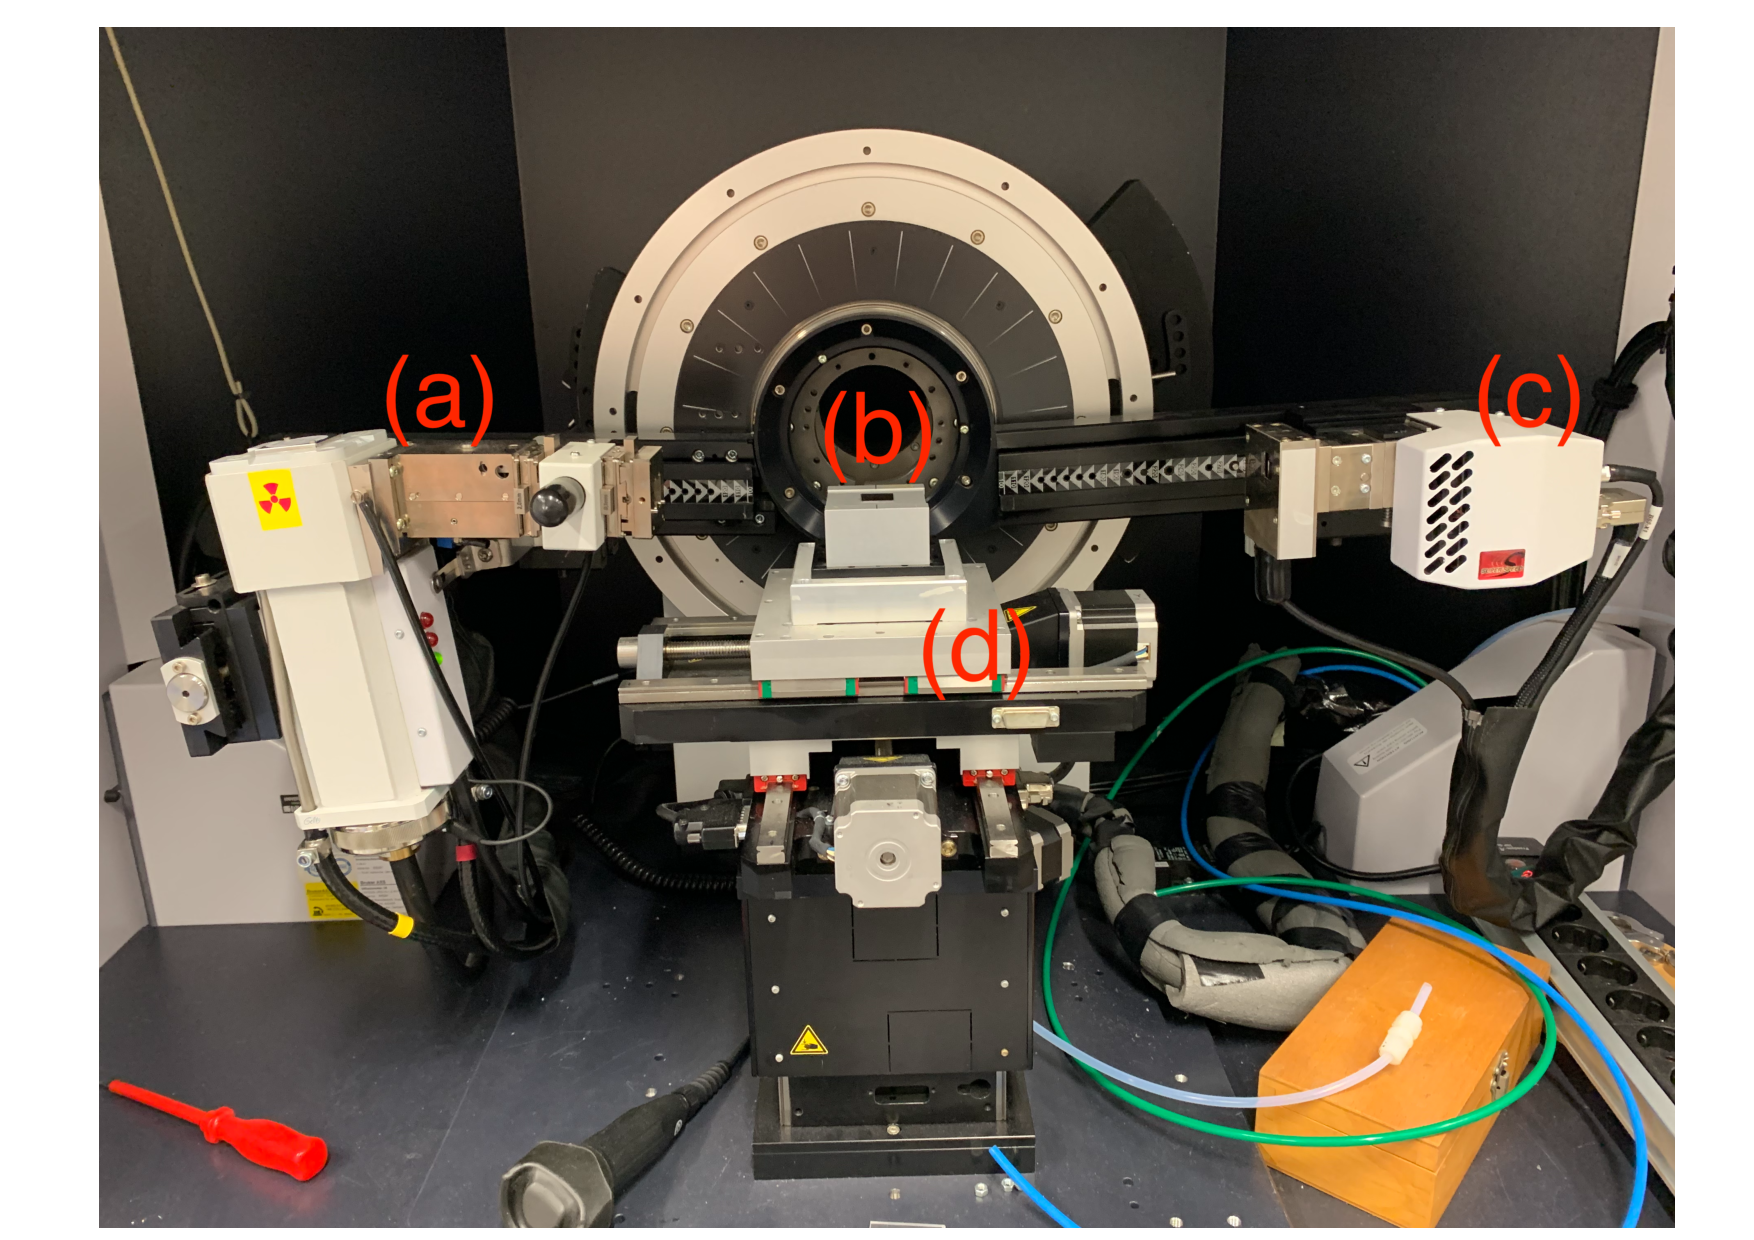
\includegraphics[scale=0.4]{content/V47_pictures/Aufbau.png}
    \caption{This figure shows the used experimental setup. \cite{v47}}
    \label{fig:aufbau}
\end{figure}
\autoref{fig:aufbau} shows the experimental setup that is used. To measure the wanted temperature dependent effects 
on the heat capacity, very low temperatures have to be achieved. \\
the copper sample which is to be analyzed is inside another copper shielding, which itself is within a recipient. This recipient is sealed tightly, so
there is no air exchange between the sample and the sorounding area. It again is located inside another vessel - a Dewar vessel.\\
The recipient is connected to two valves, which lead to a vacuum pump and a helium container.
To heat sample and copper shielding independelty, both have their own heating coil which can be controlled via a chosen 
heating voltage and current. The heat of the sample and copper shielding are measured with a Pt-100 measuring resistor, which
has a temperature dependent resistance. The amount of resistance is measured with an ohmmeter and the corresponding temperature
calculated with \cite{eq:resistance}.

\section{Experimental execution}

At the beginning the sample has to be cooled down to 80 K. To do this, the recipient has to be evacuated and filled with helium. To further
help with the cooling process and stop the recipient from getting heated from the outside, the Dewar vessel is carefully filled with liquid 
nitrogen. This is done with a pair of safety gloves and a hopper. This process takes up to an hour.\\
When 80 K is reached, the valve to the helium container is closed up and the vacuum pump is started again to evacuate the recipient
to minimize heat loss trough the air molecules.\\
As soon as the recipient is fully evacuated the measuring process will start. The heating coils are turned on and the value for the
heating voltage and current for the sample are chosen to be $\qty{16.56}{\volt}$ and $\qty{157.6}{\milli\ampere}$. The heating voltage and current for the shielding
are constantly adjusted, so the temperature of the shielding matches the one of the sample. This way heat loss through convection is also minimized.
Further heating loss through cable attachements (conduction) and radiation cannot be stopped, but are assumed to be very minor and will not be taken into account.\\
Every time the temperature has risen by approximately 7 to 11 K, the heating time, the heating voltage and current of the sample and the exact resistance are noted.
Every measurent takes between 5 and 8 minutes. This is repeated until the sample has reached a temperature of 300 K.